\documentclass[11pt]{article}

%  USE PACKAGES  ---------------------- 
\usepackage[margin=0.7in,vmargin=1in]{geometry}
\usepackage{amsmath,amsthm,amsfonts}
\usepackage{amssymb}
\usepackage{fancyhdr}
\usepackage{enumerate}
\usepackage{mathtools}
\usepackage{hyperref,color}
\usepackage{enumitem,amssymb}
\newlist{todolist}{itemize}{4}
\setlist[todolist]{label=$\square$}
\usepackage{pifont}
\newcommand{\cmark}{\ding{51}}%
\newcommand{\xmark}{\ding{55}}%
\newcommand{\done}{\rlap{$\square$}{\raisebox{2pt}{\large\hspace{1pt}\cmark}}%
\hspace{-2.5pt}}
\newcommand{\HREF}[2]{\href{#1}{#2}}
\usepackage{textcomp}
\usepackage{listings}
\lstset{
basicstyle=\small\ttfamily,
% columns=flexible,
upquote=true,
breaklines=true,
showstringspaces=false
}
%  -------------------------------------------- 

%  HEADER AND FOOTER (DO NOT EDIT) ----------------------
\newcommand{\problemnumber}{0}
\pagestyle{fancy}
\fancyhead{}
\fancyhead[L]{\textbf{Question \problemnumber}}
\newcommand{\newquestion}[1]{
\clearpage % page break and flush floats
\renewcommand{\problemnumber}{#1} % set problem number for header
\phantom{}  % Put something on the page so it shows
}
\fancyfoot[L]{IE 332}
\fancyfoot[C]{Assignment submission}
\fancyfoot[R]{Page \thepage}
\renewcommand{\footrulewidth}{0.4pt}

%  --------------------------------------------


%  COVER SHEET (FILL IN THE TABLE AS INSTRUCTED IN THE ASSIGNMENT) ----------------------
\newcommand{\addcoversheet}{
\clearpage
\thispagestyle{empty}
\vspace*{0.5in}

\begin{center}
\Huge{{\bf IE332 Project \#2}} % <-- replace with correct assignment #

Due: April 28th, 11:59pm EST % <-- replace with correct due date and time
\end{center}

\vspace{0.3in}

\noindent We have {\bf read and understood the assignment instructions}. We certify that the submitted work does not violate any academic misconduct rules, and that it is solely our own work. By listing our names below we acknowledge that any misconduct will result in appropriate consequences. 

\vspace{0.2in}

\noindent {\em ``As a Boilermaker pursuing academic excellence, I pledge to be honest and true in all that I do.
Accountable together -- we are Purdue.''}

\vspace{0.3in}

\begin{table}[h!]
  \begin{center}
    \label{tab:table1}
    \begin{tabular}{c|m{5em}m{5em}m{5em}m{5em}m{4em}|c|c}
      Student & Algorithm Development & Complexity Analysis & Implementation & Performance Analysis/Testing & A5 & Report & Overall & DIFF\\
      \hline
      Annie Zhang & 10 & 60 & 10 & 10 & 10 & 100 & 0\\
      Caroline Cudney & 10 & 10 & 60 & 10 & 60 & 100 & 0\\
      Hrishabh Nadkarni & 60 & 10 & 10 & 10 & 10 & 100 & 0\\
      Mounzr Nabulsi & 10 & 10 & 10 & 10 & 10 & 50 & 50\\
      Yuze Tang & 10 & 10 & 10 & 60 & 10 & 70 & 30\\
      \hline
      St Dev & 20 & 20 & 20 & 20 & 20 & 44.27 & 44.27
    \end{tabular}
  \end{center}
\end{table}

\vspace{0.2in}

\noindent Date: \today.
}
%  -----------------------------------------

%  TODO LIST (COMPLETE THE FULL CHECKLIST - USE AS EXAMPLE THE FIRST CHECKED BOXES!) ----------------------
\newcommand{\addtodo}{
\clearpage
\thispagestyle{empty}

\section*{Read Carefully. Important!}

\noindent By electronically uploading this assignment to Brightspace you acknowledge these statements and accept any repercussions if in any violation of ANY Purdue Academic Misconduct policies. You must upload your homework on time for it to be graded. No late assignments will be accepted. {\bf Only the last uploaded version of your assignment before the due date will be graded}.

\vspace{0.2in}

\noindent {\bf NOTE:} You should aim to submit no later than 30 minutes before the deadline, as there could be last minute network traffic that would cause your assignment to be late, resulting in a grade of zero. 

\vspace{0.2in}

\noindent When submitting your assignment it is assumed that every student considers the below checklist, as there are grading consequences otherwise (e.g., not submitting a cover sheet is an automatic grade of ZERO).

\begin{todolist}

    \item[\done] Your solutions were prepared using the \LaTeX template provided in Brightspace. 
    \item[\done] Your submission has a cover sheet as its first page and this checklist as its second page, according to the template provided.
	 \item All of your solutions (program code, etc.) are included in the submission as requested. % Check this checkbox and the following ones if satisfied <---
    \item You have not included any screen shots, photos, etc. (plots should be intermediately saved as .png files and then added into your .tex file). % <---
	 \item All math notation and algorithms (algorithmic environment) are created using appropriate \LaTeX code (no pictures, handwritten solutions, etc.). % <---
    \item The .pdf is submitted as an individual file and not in a {\tt .zip}.
    \item You kept the \LaTeX source code in your files until this assignment is graded, in case you are required to show proof of creating your assignment using \LaTeX.  % <---
    \item If submitting with a partner, your partner is added in the submission section in Gradescope after you upload your file. % <---
    \item You have correctly matched each question to its page \# in the .pdf submission in the Gradescope section (after you uploaded your file).
    \item Watch videos on creating pseudocode if you need a refresher or quick reference to the idea. These are good starter videos:    % <---
    
     \HREF{https://www.youtube.com/watch?v=4jLO0vXPktU}{www.youtube.com/watch?v=4jLO0vXPktU} 
    
    \HREF{https://www.youtube.com/watch?v=yGvfltxHKUU}{www.youtube.com/watch?v=yGvfltxHKUU}
\end{todolist}
}

%% LaTeX
% Für alle, die die Schönheit von Wissenschaft anderen zeigen wollen
% For anyone who wants to show the beauty of science to others

%  -----------------------------------------


\begin{document}


\addcoversheet
\addtodo

% BEGIN YOUR ASSIGNMENT HERE:
\newquestion{Table of Contents}

%TABLE OF CONTENTS
\tableofcontents

%MAIN TEXT OF REPORT
\pagebreak
\newquestion{Report}
\section{Background}
Binary classifiers are a type of supervised machine learning algorithms that are used to split objects into one of two groups or classes. They are often used in medical evaluations when diagnosing a patient as positive or negative and have other applications including email spam and quality assurance. The binary classifier for this project focuses on identifying whether images were showing dandelions or just grass by computing a percentage. The code outputs two separate percents per image. The first percent is the amount it predicts that the image is a dandelion, and the second percent is the amount the algorithm predicts the image is of grass. If it is over 50 for the first percent, then the algorithm declares that the image is of dandelions, otherwise it says it is grass because the second percent would then be over 50. The goal of the project is to implement algorithms before running the binary classifier that are adversarial attacks altering the images to fool it, so the classifier always identifies the image as grass even when that isn't true. The adversarial attacks add noise to the images, but the noise shouldn't disrupt the image to the extent that the viewer also can't tell what it is or classify it correctly. An example image is shown below.\\
\begin{center}
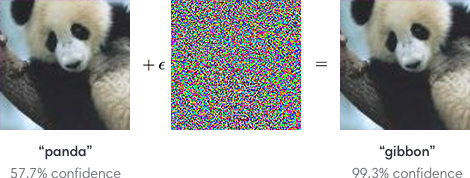
\includegraphics[scale=.75]{attackidea.png}\\
\end{center}
Adversarial attacks can be problematic in the real world because they affect the validity and usefulness of classifiers. The attacks alter the results decreasing the accuracy and causing incorrect conclusions that can be harmful, especially depending on the initial use of the classifier. It may flag an important email as spam, let a faulty product be sold, or cause a patient to receive proper care. Understanding and being able to recognize and avoid adversarial attacks can help to ensure that classifiers are able to appropriately and accurately do their job. They can be combated by using detectors or separate models rejecting adversarial examples. One can also implement preprocessing, denoising, and principal component analysis. Lastly, to fight adversarial attacks, adversarial training can be used, which is training with adversarial examples, so the model is more prepared, \\
There are white box and black box adversarial attacks both working to fool neural networks into making incorrect conclusions by adding noise, but white box attacks allow for complete access to the architecture, input, and output of the model while black box only allows access to the model input and output. The different attack types employed in this project were found through researching and comparing. In the end, five algorithms were chosen including FGSM, DeepFool, Partcile Swarm, CW, and PGD. These use different approaches of adding noise including finding and applying the smallest possible perturbations as well as taking small gradient steps. Other potential algorithms that could have been used include hill climbing or simulated annealing. \\
The different algorithms were then coded into R and placed into the given code for the model to be tested and analyzed. The algorithms were tried individually then combined and weighted to be tested together. The rest of the report after detailing the different algorithms shows the testing, correctness, verification, computation complexity with run time and walltime, and overall performance. \\
https://viso.ai/deep-learning/adversarial-machine-learning/
https://deepchecks.com/glossary/binary-classification/ - info 
\addcontentsline{toc}{section}{Algorithm 1}
\section*{Algorithm 1}
FGSM Algorithm\\
The fast gradient sign method is a white box attack with a goal of misclassification. It calculates the losses after forward propagation, then calculates the gradient with respect to the image pixels, and finally adjusts the pixels of the images slightly in the direction of the gradients maximizing the loss. \\
https://neptune.ai/blog/adversarial-attacks-on-neural-networks-exploring-the-fast-gradient-sign-method 
https://neptune.ai/blog/adversarial-attacks-on-neural-networks-exploring-the-fast-gradient-sign-method
\addcontentsline{toc}{section}{Algorithm 2}
\section*{Algorithm 2}
DeepFool Algorithm\\
This algorithm is a type of white box attack algorithm that adds the minimum necessary perturbations to an image that will change the classification label. The pseudocode for the algorithm can be seen below. \\
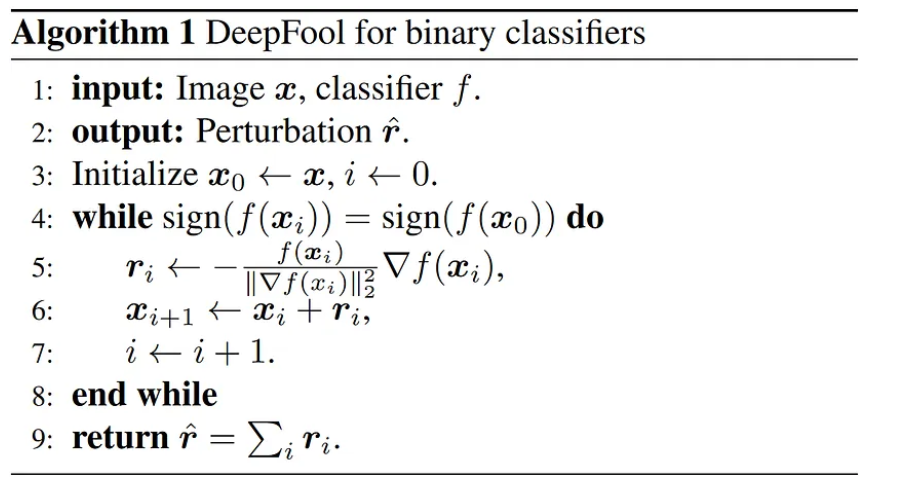
\includegraphics[scale=.5]{deepfoolpseudo.png} \\
https://towardsdatascience.com/deepfool-a-simple-and-accurate-method-to-fool-deep-neural-networks-17e0d0910ac0
https://medium.com/machine-intelligence-and-deep-learning-lab/a-review-of-deepfool-a-simple-and-accurate-method-to-fool-deep-neural-networks-b016fba9e48e
https://www.crcv.ucf.edu/wp-content/uploads/2018/11/Lecture-3-DeepFool.pdf
https://ebezzam.github.io/pdf/lts4_semester_project_eric_bezzam.pdf

\addcontentsline{toc}{section}{Algorithm 3}
\section*{Algorithm 3}
Particle Swarm Optimization\\
This particle swarm optimization algorithm operates by finding the local optima and changing them until the classifier can be successfully fooled. The pseudocode for this algorithm is displayed below. \\
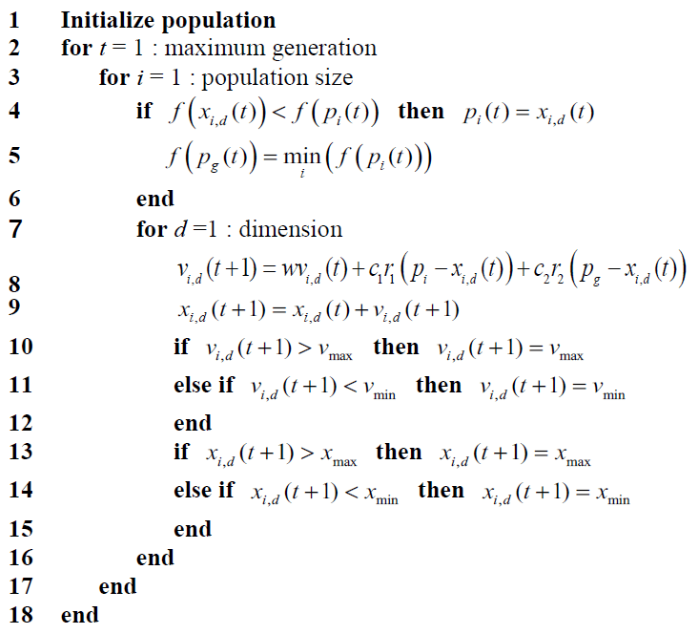
\includegraphics[scale=.5]{particleswarmpseudo.png} \\
https://www.researchgate.net/figure/Pseudocode-of-standard-particle-swarm-optimization_fig1_323281605
https://rpubs.com/argaadya/intro-pso
https://www.analyticsvidhya.com/blog/2021/10/an-introduction-to-particle-swarm-optimization-algorithm/

\addcontentsline{toc}{section}{Algorithm 4}
\section*{Algorithm 4}
CW Algorithm\\
The Carlini Wagner algorithm is an iterative attack adding perturbations to increase the chance that the image is incorrectly classified. \\
https://www.skillsire.com/read-blog/359_a-overview-on-adversarial-attacks-and-defenses.html
\addcontentsline{toc}{section}{Algorithm 5}
\section*{Algorithm 5}
PGD Algorithm \\
Projected gradient descent is an algorithm similar to FGSM; however, it calculates a new gradient each iteration with smaller perturbations helping to choose a more ideal stepping size for the attack. \\
https://www.skillsire.com/read-blog/359_a-overview-on-adversarial-attacks-and-defenses.html

% Testing/Correctness/Verification
\section{Testing/Correctness/Verification}
Each algorithm was tested, analyzed for correctness, and verified to ensure it was properly functioning.
\addcontentsline{toc}{section}{Algorithm 1}
\section*{Algorithm 1}
\addcontentsline{toc}{section}{Algorithm 2}
\section*{Algorithm 2}
\addcontentsline{toc}{section}{Algorithm 3}
\section*{Algorithm 3}
\addcontentsline{toc}{section}{Algorithm 4}
\section*{Algorithm 4}
\addcontentsline{toc}{section}{Algorithm 5}
\section*{Algorithm 5}


\section{Runtime Complexity and Walltime}
Runtime complexity analyzes the computational complexity of an algorithm to develop an idea of how long it will take to run based on a function for the input size n. For this, the input n would be the number of iterations determined by the number of pixels the algorithm must change before the classifier is finally fooled. Walltime is the actual numerical time the algorithm took when running calculated by a clock.
\\
A lower runtime and walltime is preferred because it is not convenient nor efficient to have to wait long periods of time for an output. There is usually a tradeoff in complexity and runtime, especially when considering the number of iterations, so it is important to consider this when developing algorithms. The amount of time can also depend on the technology one is using, so investing in better, more advanced technology may be helpful in reducing the wait time and allow for more complex algorithms to take less time. \\
\addcontentsline{toc}{section}{Algorithm 1}
\section*{Algorithm 1}
\addcontentsline{toc}{section}{Algorithm 2}
\section*{Algorithm 2}
\addcontentsline{toc}{section}{Algorithm 3}
\section*{Algorithm 3}
\addcontentsline{toc}{section}{Algorithm 4}
\section*{Algorithm 4}
\addcontentsline{toc}{section}{Algorithm 5}
\section*{Algorithm 5}


\section{Performance}
The overall performance of the algorithms was analyzed to see how well they worked and their efficiency. It is important that 
\addcontentsline{toc}{section}{Algorithm 1}
\section*{Algorithm 1}
\addcontentsline{toc}{section}{Algorithm 2}
\section*{Algorithm 2}
\addcontentsline{toc}{section}{Algorithm 3}
\section*{Algorithm 3}
\addcontentsline{toc}{section}{Algorithm 4}
\section*{Algorithm 4}
\addcontentsline{toc}{section}{Algorithm 5}
\section*{Algorithm 5}


\begin{lstlisting}[language=R, frame=single]
#Algorithm 1
x <- c(1,2,3)
\end{lstlisting}
\begin{lstlisting}[language=R, frame=single]
#Algorithm 2
x <- c(1,2,3)
\end{lstlisting}
\begin{lstlisting}[language=R, frame=single]
#Algorithm 3
x <- c(1,2,3)
\end{lstlisting}
\begin{lstlisting}[language=R, frame=single]
#Algorithm 4
x <- c(1,2,3)
\end{lstlisting}
\begin{lstlisting}[language=R, frame=single]
#Algorithm 5
x <- c(1,2,3)
\end{lstlisting}
\end{document}
